%SourceDoc ../YourName-Dissertation.tex
\vspace*{-80mm}
\chapter{Shock Tube} \label{chapter5:Shock_Tube}
 
	\section{Problem Setup} \label{Verification:Shock_Tube}
        
    A shock tube is a very common and standard method of verification for
    momentum and pressure. However, an exact analytical solution is more readily
    obtained for an ideal gas such as air. A shock tube is created by setting
    the initial mass flow rate and velocity to zero with no gravity. The
    boundary conditions at the inlet and outlet are also set to zero, simulating
    a closed system. A region of high pressure is defined for one half of the
    domain, and a region of low pressure for the second half. An imaginary
    diaphragm divides the two regions before the simulation, and at $t=0$
    disappears.
    
    \begin{figure}[!h]
    	\centering
    	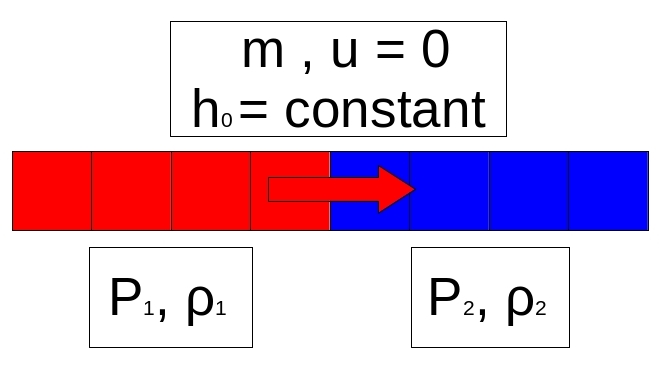
\includegraphics[width=0.55\textwidth]{images/Verification_Problem2_shock_tube}
    	\label{fig:Verification_2}
    	\caption{Setup for the shock tube problem}
    \end{figure}
    
    The problem was set up using the parameters given in table
    \ref{table:ST_Params}. The geometry is similar to the previous problem, but
    the length of the tube was elongated to take into account the faster
    propagation of the rarefaction and compression waves. The temperature and
    pressure of the air are near standard conditions.
    
    \begin{table}[!h]
    	\center
    	\label{table:ST_Params}
    	\caption{Input Parameters for Shock Tube Verification Problem}
    	\begin{tabular}{|c|c|c|}
    		\hline
	    	Length 	  				&  25.00	& m 		\\ \hline 
	    	Channel Area			&  0.0001	& $m^{2}$	\\ \hline
	    	Wetted Perimeter		&  0.040	& m			\\ \hline
	    	Initial Pressure  		&  1.00		& bar		\\ \hline
	    	Initial Enthalpy		&  304.66575& kJ/kg		\\ \hline
	    	Initial Mass Flow Rate 	&  0.000	& kg/s		\\ \hline
	    	Initial Pressure Drop	&  0.09576  & bar 		\\ \hline
    	\end{tabular}
    \end{table}    
    
    Each region has a unique density corresponding to the different pressures
    using the equation of state for air given in equation \ref{eq:EOS_air} where $\gamma
    = 1.4$ is the ratio of specific heats for air. Additionally, the specific
    heat $Cp = 1.005 \frac{kJ}{kg-K}$ to convert between enthalpy and
    temperature. The initial enthalpy of the system is constant, but will change
    non-uniformly as a function of time. The velocity is initially set to zero,
    but will change as the compression and rarefaction waves move. Since the
    velocity is set to zero initially, it can't be used to evaluate the time
    step size. Instead the speed of sound can be evaluated using equation
    \ref{eq:sound_speed}, and this velocity can be used to calculate the time
    step. While there might be some slight change in the speed of sound due to
    enthalpy changes, it should remain effectively constant.
    
    \begin{equation}
    \label{eq:EOS_air}
    	\rho = \left( \frac{\gamma}{\gamma - 1} \right) \frac{P_{abs}}{h} 
    \end{equation}
    
    \begin{equation}
    \label{eq:sound_speed}
    a = \sqrt{ \left( \gamma - 1 \right) h }
    \end{equation}
    
    \begin{equation}
    \gamma = \frac{C_{p}}{C_{v}}
    \end{equation}
    
    \section{Analytical Solution}
    
    When the diaphragm disappears, a compression wave will move to the right and a
    rarefaction wave to the left. These two waves split the domain into four
    distinct regions as shown in figure \ref{fig:V2_pressure_scaling}. 
    
    \begin{enumerate}
      \item left of the rarefaction wave
      \item between the rarefaction wave and the initial location of the diaphragm
      \item between the initial location of the diaphragm and the compression wave
      \item right of the compression wave
    \end{enumerate}
    
    The analytical solution does not take into account reflection off of the
    walls, however the numerical solution can due to the applied boundary
    conditions for mass flow rate.
    
    \begin{figure}[!h]
    	\centering
    	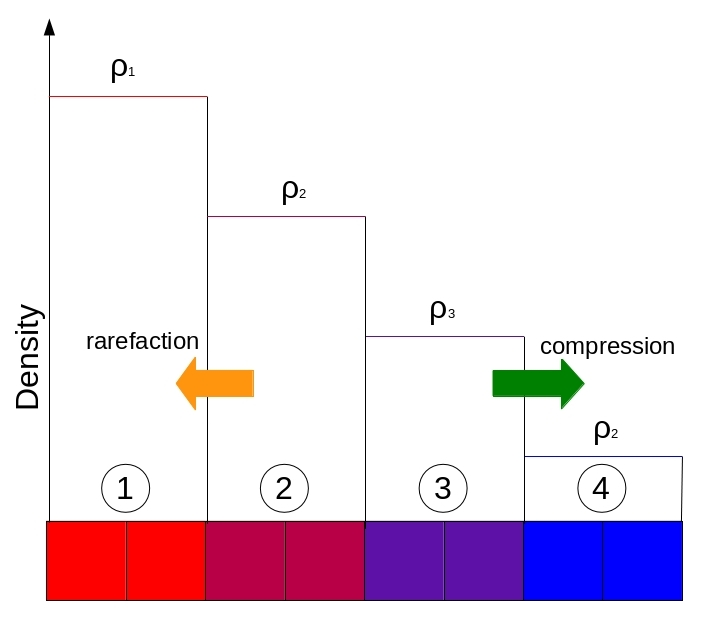
\includegraphics[width=0.50\textwidth]{images/Shock_Tube/Shock_Tube_regions}
    	\label{fig:V2_pressure_scaling}
    	\caption{Regions within the shock tube based on rarefaction and compression}
    \end{figure}
    
    For a perfectly caloric gas, the following equations are provided
    \cite[p. 238]{Anderson1990} given the initial conditions for state 1 and
    4 in conjunction with equation \ref{eq:sound_speed}. An iterative method is
    required to solve \ref{eq:ref1_7.94} for $\frac{P_{2}}{P_{1}}$. Once the region
    properties are obtained, the regions themselves are mapped by comparing the
    current position and time to the velocity of the rarefaction and compression
    wave. 
    
    \begin{equation}
    \label{eq:ref1_7.94}
    	\frac{P_{4}}{P_{1}} = \frac{P_{2}}{P_{1}} \frac{
    	\left( 1 - (\gamma-1)(\frac{a_{1}}{a_{4}})(\frac{P_{2}}{P_{1}} -1) \right) }
    	{\sqrt{2 \gamma \left[ 2 \gamma + (\gamma +1)(\frac{P_{2}}{P_{1}} -1)\right]}}^{
    	- \frac{2 \gamma}{\gamma - 1}}
    \end{equation}
    
    \begin{equation}
    	\frac{T_{2}}{T_{1}} = \frac{P_{2}}{P_{1}} \left(
    	\frac{\frac{\gamma + 1}{\gamma - 1} + \frac{P_{2}}{P_{1}}}
    	{1 + (\frac{\gamma +1}{\gamma - 1}) \frac{P_{2}}{P_{1}}} \right)
    \end{equation}
    
    \begin{equation}
    	\frac{\rho_{2}}{\rho_{1}} =
    	\frac{1 + (\frac{\gamma + 1}{\gamma - 1}) \frac{P_{2}}{P_{1}}}
    	{\frac{\gamma + 1}{\gamma - 1} + \frac{P_{2}}{P_{1}}} 
    \end{equation}
    
    \begin{equation}
    	W = a_{1} \sqrt{ \frac{\gamma + 1}{2 \gamma} 
    	                 \left( \frac{P_{2}}{P_{1}} -1 \right) +1 }
    \end{equation}
    
    \begin{equation}
    	P_{2} = P_{3}
    \end{equation}
    
    \begin{equation}
    	\frac{P_{3}}{P_{4}} = 
    	\left( \frac{\rho_{3}}{\rho_{4}} \right)^{\gamma} =
    	\left( \frac{T_{3}}{T_{4}} \right)^{\frac{\gamma}{\gamma -1}}
    \end{equation}
    
    \section{Results and Error}
    
    Enthalpy and density have a discontinuity as seen in figure
    \ref{fig:V2_result_top} where the diaphragm was initially placed . Similarly
    there are discontinuities that move with the rarefacation and compression
    waves for pressure, density, and velocity. The largest error occurs around
    these discontinuities as seen in figure \ref{fig:V2_result_bottom}. A 
    fine spatial mesh and a small time step are needed to accurately reflect the
    exact solution.
    
    \pagebreak
    \begin{figure}[!h]
    	\centering
    	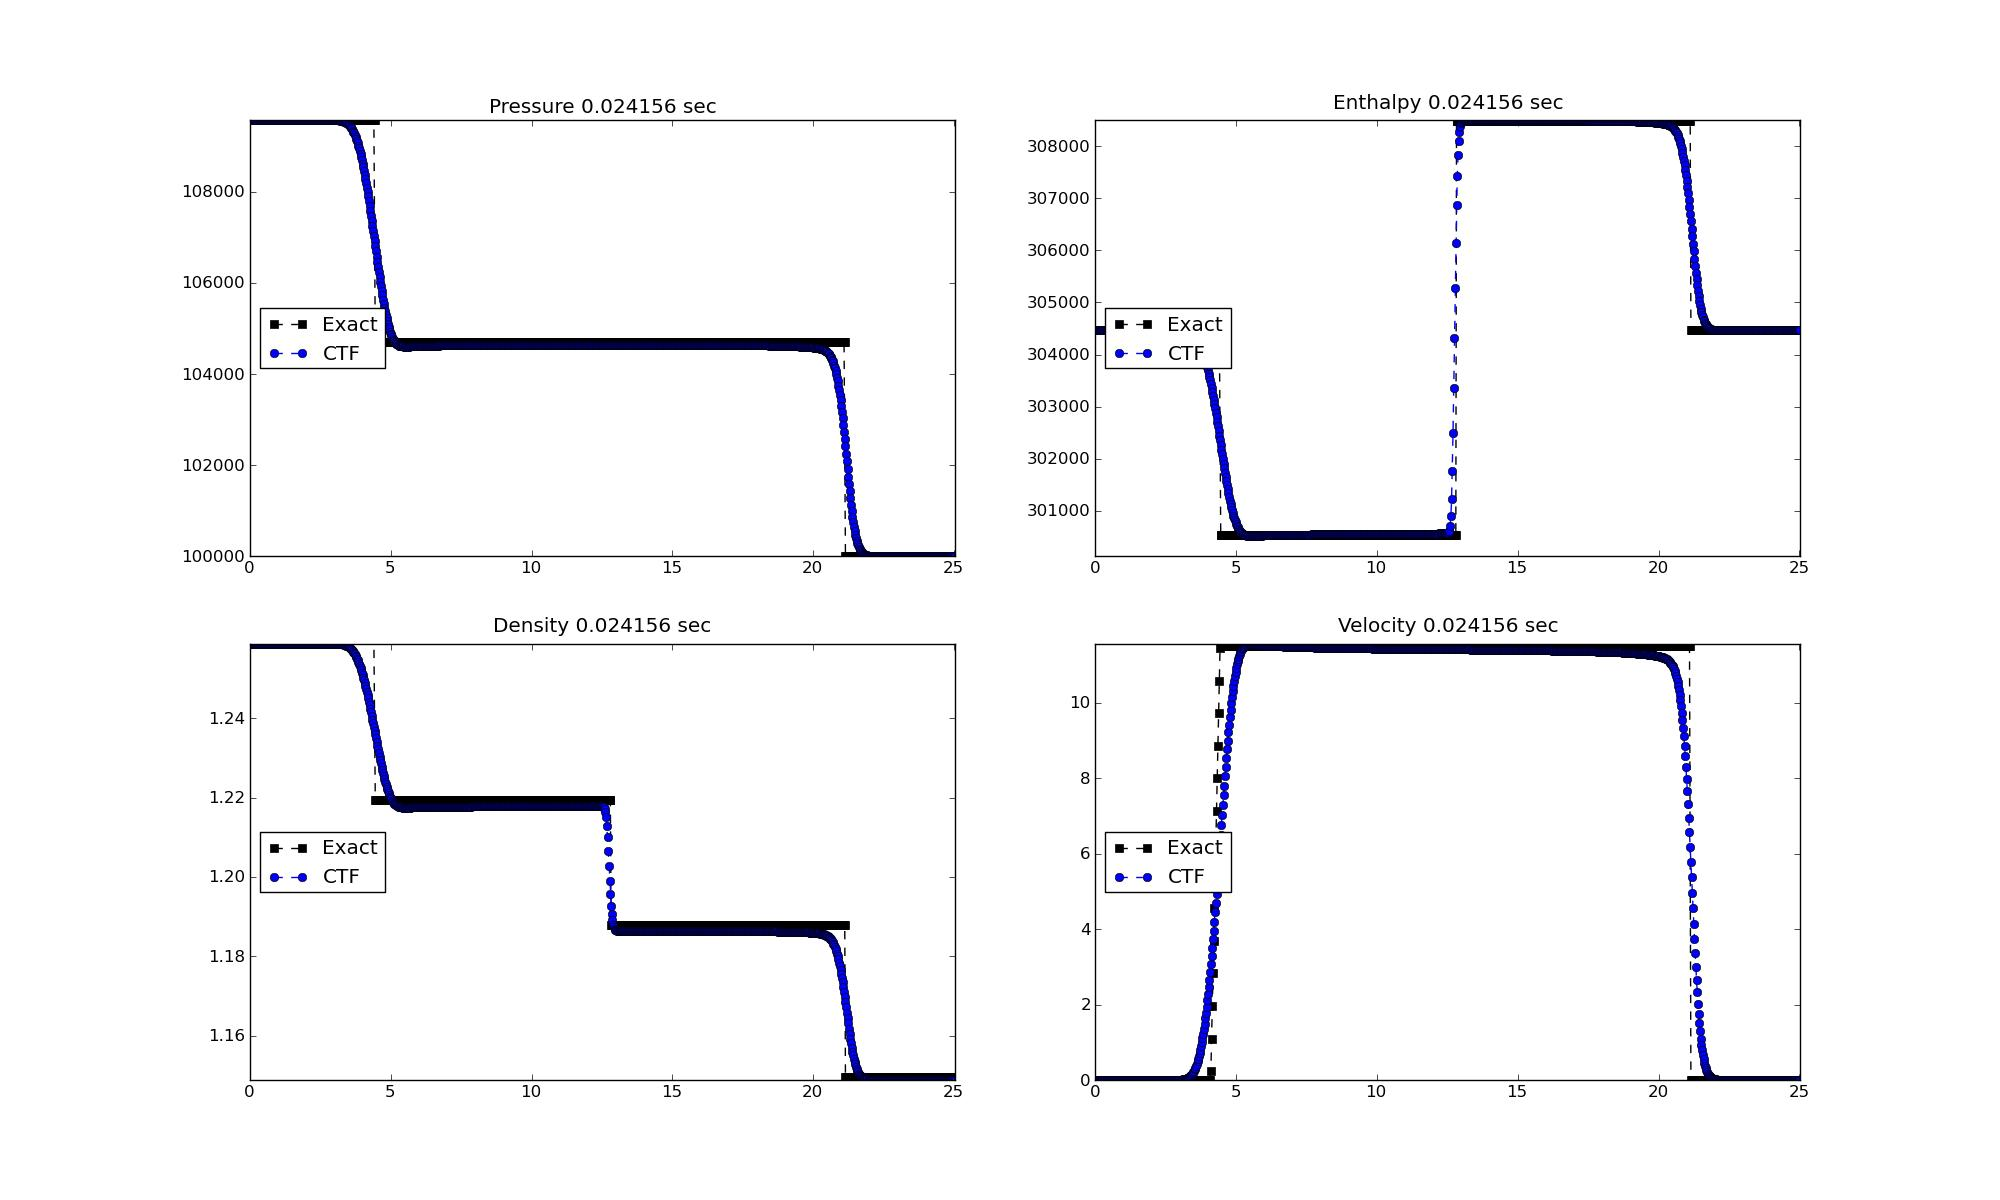
\includegraphics[width=1.30\textwidth,angle=90.0]{images/wave1_200dP_N1000/tmp/plot_shocktube_0034}
    	\caption{Comparison of analytical and numerical results for shock tube}
    	\label{fig:V2_result_top}
    \end{figure}
    
    \pagebreak
    \begin{figure}[!h]
    	\centering
    	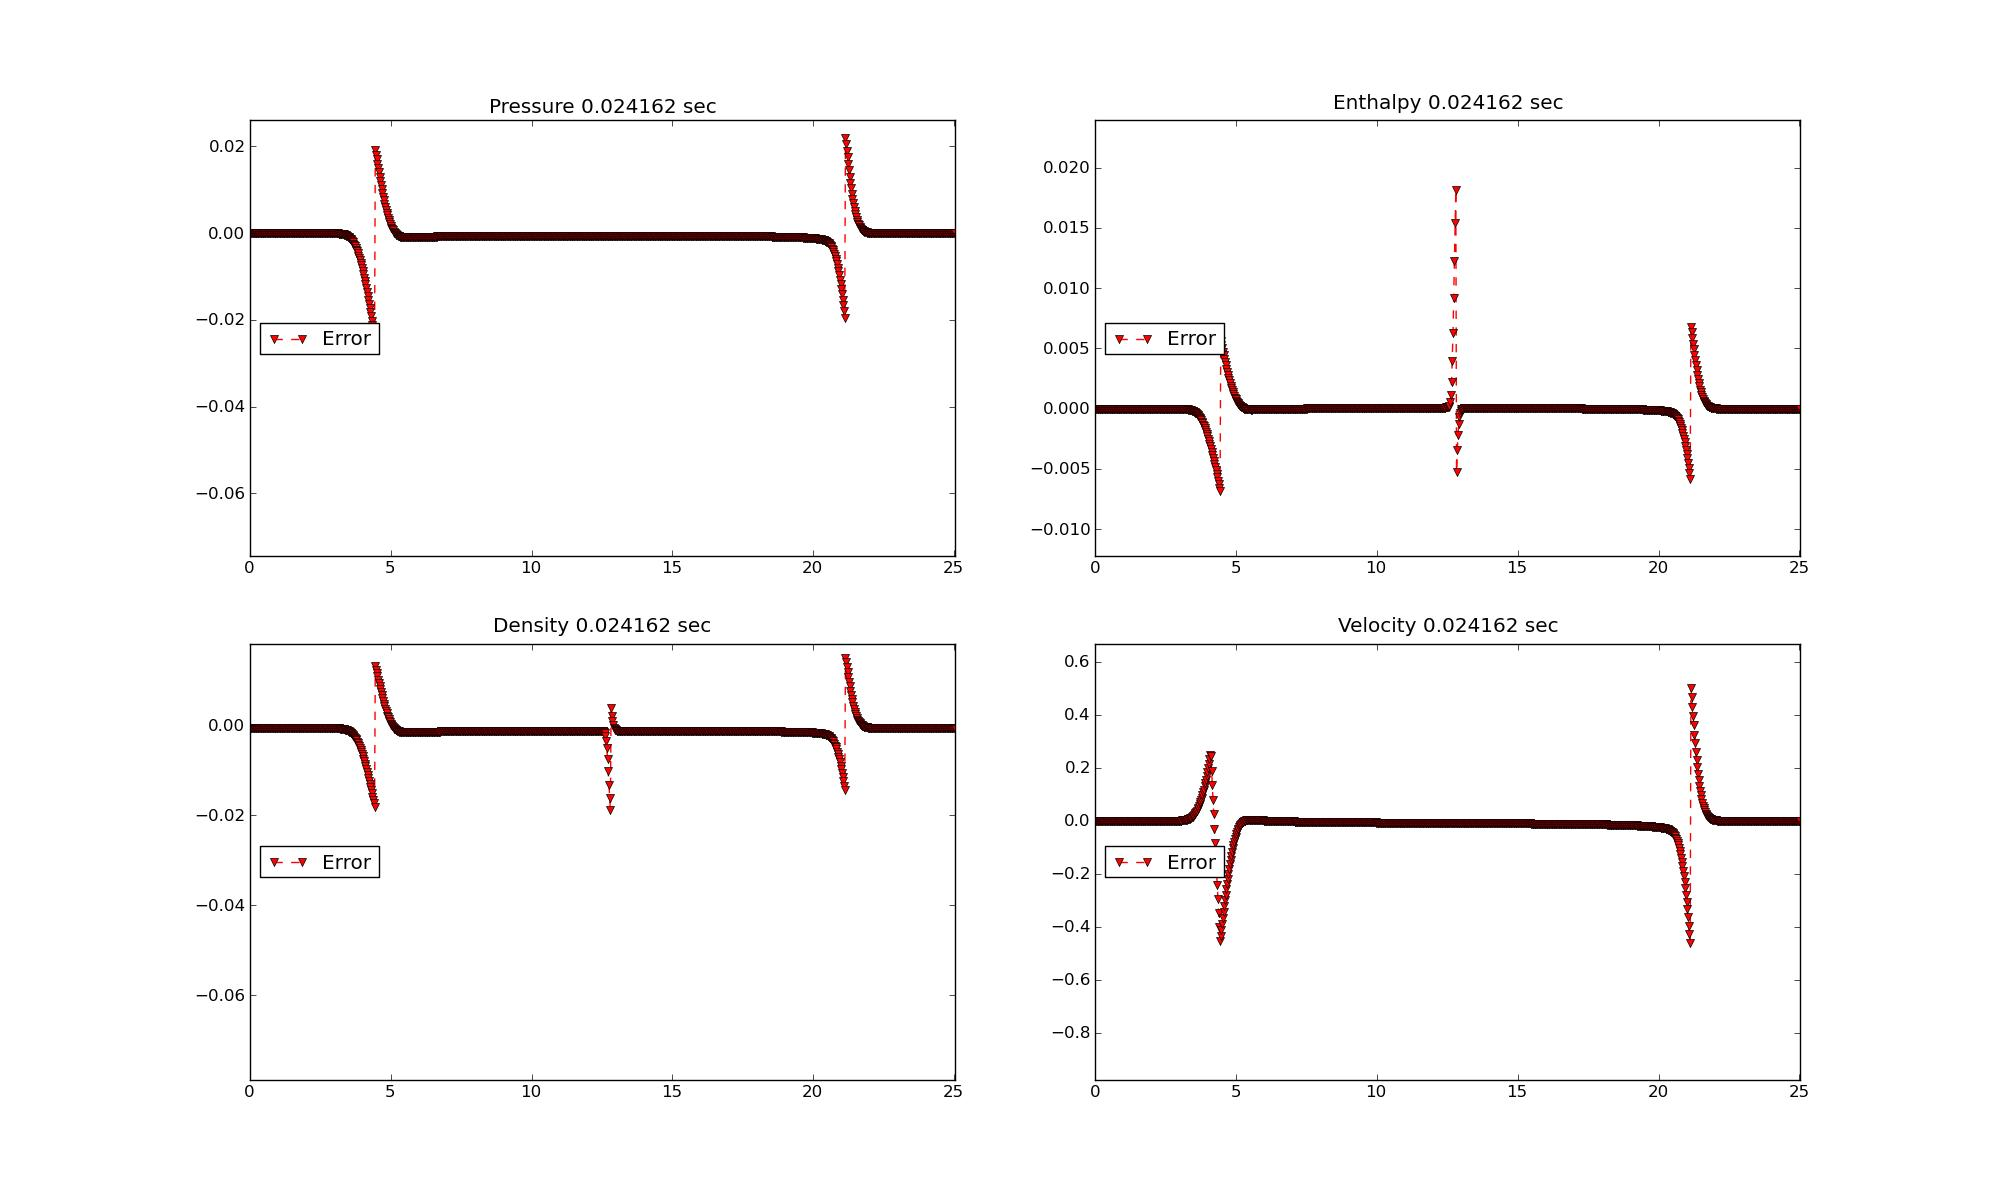
\includegraphics[width=1.30\textwidth,angle=90.0]{images/wave1_200dP_N1000/tmp/plot_st_err_0679}
    	\caption{Truncation error for shock tube}
    	\label{fig:V2_result_bottom}
    \end{figure}
    
    \pagebreak
    \section{Scaling of Error}
    
    A Richardson Extrapolation was performed on the density, enthalpy, and mass
    flow rate for the shock tube analysis in time. The error approaches zero
    as the time step size gets smaller as seen in figure
    \ref{fig:ST_Err_rho}. The order of accuracy with respect to time is
    converges to first order accurate as the time step size decreases. The range
    of time step values shown are within the asymptotic limit. 
    
    \begin{figure}[!h]
    	\centering
    	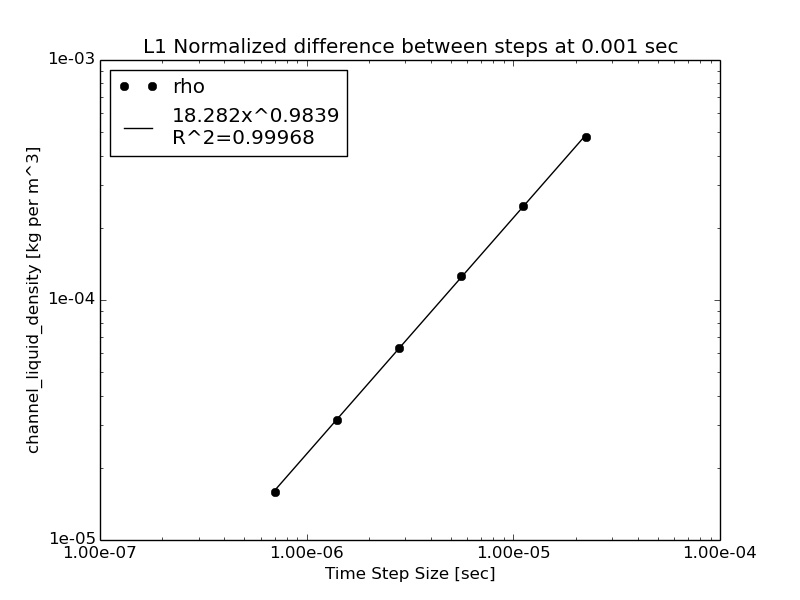
\includegraphics[width=0.5\textwidth]{images/Shock_Tube/Difference_rho}
    	\caption{Richardson Extrapolation of the shock tube results N=50}
    	\label{fig:ST_Err_rho}
    \end{figure}
    
    \begin{figure}[!h]
    	\centering
    	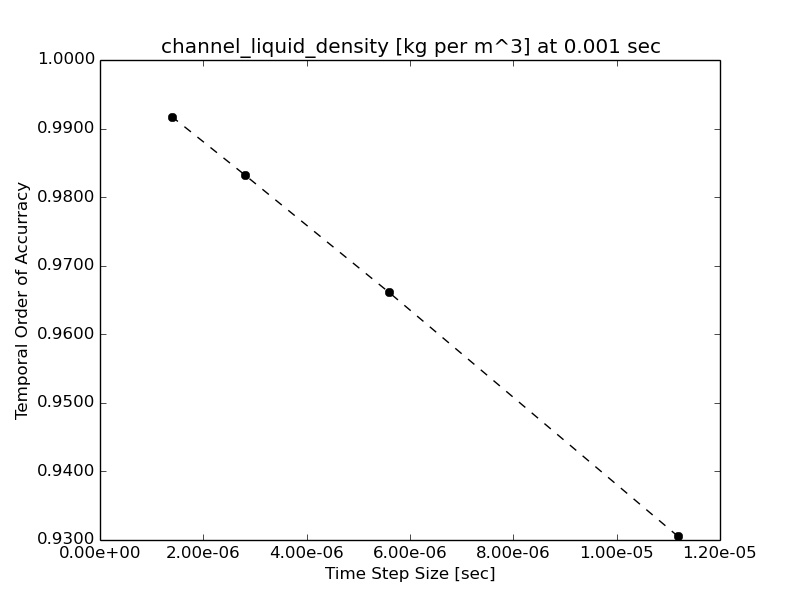
\includegraphics[width=0.50\textwidth]{images/Shock_Tube/Temporal_Order_Of_Accuracy_rho}
    	\caption{Temporal Order of Accuracy for shock tube}
    	\label{fig:ST_OOA_rho}
    \end{figure}
	
	
